\part{States}
    \section{Quantum States}
    \subsection{Classical States}
    In classical mechanics a point like system's state is entirely described by two 3-dimensional vectors, namely position, \(\vv x\), and momentum, \(\vv p\).
    These are 3-dimensional real vectors living in \(\reals^3\).
    We can instead view the object \((\vv x, \vv p)\) as a 6-dimensional real vector living in \(\reals^6\).
    In this way we can completely describe the state of the system with one 6-dimensional vector.
    By this we mean that using \((\vv x, \vv p)\) and Newton's laws we can compute the time evolution of the system, that is what the state will be at some time in the future, or what the state was at some time in the past.
    We can also compute other values such as energy and angular momentum, these are observables that we can measure along with position and momentum.
    
    \subsection{Quantum States}
    In \acrfull{qm} the state of a system can also be encoded in a single vector, although the way that we do this is more complex (literally).
    We start with the following postulate:
    \begin{postulate}\label{pos:quantum state is complex vector}
        The state of a quantum system is described by a complex vector.
    \end{postulate}
    In classical mechanics the state vector is real and therefore composed of values that can be measured.
    In \acrshort{qm} we cannot directly measure the components of this complex vector.
    The way we measure observables will be covered in detail later.
    For now we focus on the mathematical side of this statement.
    
    In this course we will use Dirac notation in which a vector is represented by \(\ket{v}\), called a \define{ket}, where \(v\) is some label.
    For example we may use \(\ket{v}\), \(\ket{\uparrow}\), or \(\ket{n, m}\).
    Here \(v\), \(\uparrow\), and \(n, m\) are simply whatever label is best suited to the problem at hand.
    
    \subsubsection{Vector Spaces}\label{sec:vector spaces}
    Our intuition for what is a vector is normally that it is some object with magnitude and direction.
    This definition fails when it comes to complex vectors and is not very useful for vectors of more than 3-dimensions.
    To be mathematically precise a \define{vector} is any element of a vector space, \(\hilbert\).
    This simply moves the problem on to the next definition, what is a vector space?
    
    A \define{vector space}, \((\hilbert, \mathbb{F}, +, \cdot)\), over a field, \(\mathbb{F}\), is a set, \(\hilbert\) and two operations, \(+\) and \(\cdot\).
    We will restrict ourselves to \(\mathbb{F} = \reals, \complex\).
    In the former case we get a real vector space and in the later a complex vector space.
    These operations are
    \begin{itemize}
        \item Vector addition, \({+}\colon\hilbert\times\hilbert\to\hilbert\), which takes two vectors, \(\ket{u}, \ket{v}\in\hilbert\) and maps them to a third vector \(\ket{u} + \ket{v}\in\hilbert\).
        \item Scalar multiplication, \({\cdot}\colon\mathbb{F}\times\hilbert\to\hilbert\), which takes a vector, \(\ket{v}\in\hilbert\), and a scalar, \(\lambda\in\mathbb{F}\), and maps them to a second vector \(\lambda\ket{v}\).
    \end{itemize}
    These operations must satisfy the following properties:
    \begin{itemize}
        \item Associativity of vector addition -- For all \(\ket{u}, \ket{v}, \ket{w}\in\hilbert\)
        \[\ket{u} + (\ket{v} + \ket{w}) = (\ket{u} + \ket{v}) + \ket{w}.\]
        In other words the bracketing around vector addition doesn't matter, the result is the same however it is bracketed.
        This is true for more than three terms being added as well.
        \item Commutativity of vector addition -- For all \(\ket{u}, \ket{v}\in\hilbert\)
        \[\ket{u} + \ket{v} = \ket{v} + \ket{u}.\]
        In other words the order of terms in a sum doesn't matter, the result is the same either way.
        \item Existence of an additive identity -- There exists \(\ket{0}\in\hilbert\) such that 
        \[\ket{0} + \ket{v} = \ket{v}\]
        for all \(\ket{v}\in\hilbert\).
        \(\ket{0}\) is called the zero vector.
        Be careful as \(\ket{0}\) may not always denote the zero vector, for example, if we use \(\ket{p}\) to denote a state with momentum \(p\) then \(\ket{0}\) denotes a state with no momentum.
        This doesn't mean that this is the zero vector.
        \item Existence of additive inverses -- For all \(\ket{v}\) there exists \(-\ket{v}\in\hilbert\) such that
        \[\ket{v} + (-\ket{v}) = \ket{0}\]
        where \(\ket{0}\) is the zero vector.
        We normally shorten this to
        \[\ket{v} - \ket{v} = \ket{0}.\]
        \item Compatibility of scalar and field multiplication -- for all \(\lambda, \mu\in\mathbb{F}\) and \(\ket{v}\in\hilbert\) we have
        \[(\lambda\mu)\ket{v} = \lambda(\mu\ket{v})\]
        here the product \(\lambda\mu\) is computed using multiplication as defined in \(\mathbb{F}\) and \(\mu\ket{v}\) and \(\lambda(\mu\ket{v})\) are computed using scalar multiplication as defined for our vector space.
        \item Identity of scalar multiplication -- If \(1\in\mathbb{F}\) is the multiplicative identity of \(\mathbb{F}\) then
        \[1\ket{v} = \ket{v}\]
        for all \(\ket{v}\in\hilbert\).
        \item Distributivity of scalar multiplication over vector addition -- For all \(\ket{u}, \ket{v}\in\hilbert\) and \(\lambda\in\mathbb{F}\)
        \[\lambda(\ket{u} + \ket{v}) = \lambda\ket{u} + \lambda\ket{v}.\]
        \item Distributivity of scalar multiplication over field addition -- For all \(\lambda, \mu\in\mathbb{F}\) and \(\ket{v}\in\hilbert\)
        \[(\lambda + \mu)\ket{v} = \lambda\ket{v} + \mu\ket{v}.\]
    \end{itemize}
    The important take away here is that for a complex vector space, \(\hilbert\) if \(\ket{u}, \ket{v}\in\hilbert\) and \(\alpha, \beta\in\complex\) then
    \[\alpha\ket{u} + \beta\ket{v} \in \hilbert.\]
    That is \(\hilbert\) is closed under vector addition and scalar multiplication.
    This easily generalises to \(\ket{v_i}\in\hilbert\) and \(\alpha_i\in\hilbert\) so
    \[\sum_i\alpha_i\ket{v_i}\in\hilbert\]
    Any linear combination of vectors is again a vector.
    
    \begin{example}
        Let \(\ket{u}\) and \(\ket{v}\) be vectors with two complex components:
        \[
            \ket{u} =
            \begin{pmatrix}
                u_1\\ u_2
            \end{pmatrix}
            ,\qquad\text{and}\qquad\ket{v} = 
            \begin{pmatrix}
                v_1\\ v_2
            \end{pmatrix}
        \]
        where \(u_1, u_2, v_1, v_2\in\complex\).
        If we define the sum of these two vectors to be
        \[
            \ket{u} + \ket{v} = 
            \begin{pmatrix}
                u_1 + v_1\\ u_2 + v_2
            \end{pmatrix}
            .
        \]
        The addition on the left hand side is vector addition, the addition on the right hand side is field addition in \(\complex\).
        We define scalar multiplication by \(\lambda\in\complex\) as
        \[
            \lambda\ket{v} =
            \begin{pmatrix}
                \lambda v_1\\ \lambda v_2
            \end{pmatrix}
            .
        \]
        Multiplication on the left hand side is scalar multiplication, multiplication on the right hand side is field multiplication in \(\complex\).
        The set, \(\complex^2\), of all such objects with this definition of vector addition and scalar multiplications is a complex vector space.
        We will use this throughout this section to give examples.
    \end{example}
    The fact that a linear combination of vectors is again a vector means that a linear combination of quantum states is again a quantum state.
    This is called the \define{superposition principle}.
    It is a direct consequence of postulate~\ref{pos:quantum state is complex vector} and the closure of vector spaces under addition and multiplication.
    In fact it is possible to state the superposition principle as the first postulate and then derive that the states need to be elements of a vector space.
    
    \subsubsection{Scalar Products}
    The scalar product, or inner product, is a function:
    \begin{align*}
        \cdot\colon\hilbert\times\hilbert &\to \complex\\
        \ket{u}, \ket{v} &\mapsto \braket{u}{v} = z\in\complex.
    \end{align*}
    The inner product also satisfies the following two properties:
    \begin{itemize}
        \item Conjugate symmetry -- For all \(\ket{u}, \ket{v}\in\hilbert\)
        \[\braket{u}{v} = \braket{v}{u}^*\]
        where \(^*\) denotes complex conjugation.
        \item Linearity in the second argument -- For all \(\ket{u}, \ket{v}, \ket{w}\in\hilbert\) and \(\alpha, \beta\in\complex\)
        \[\bra{u}\left[\alpha\ket{v} + \beta\ket{w}\right] = \alpha\braket{u}{v} + \beta\braket{u}{w}.\]
    \end{itemize}
    Combining these properties we get that for all \(\ket{u}, \ket{v}, \ket{w}\in\hilbert\) and \(\alpha, \beta\in\complex\)
    \[\left[\alpha\bra{u} + \beta\bra{v}\right]\ket{w} = \alpha^*\braket{u}{w} + \beta^*\braket{v}{w}.\]
    A vector space equipped with an inner product is called a \define{Hilbert space}.\footnote{Technically it is just an inner product space, a Hilbert space is then an inner product space that is Cauchy complete. That is all series of vectors that converge absolutely (the sum of the norms of the vectors converges) in \(\hilbert\) converge (the sum of the vectors converges) in \(\hilbert\). However all inner product spaces can be extended to be Hilbert spaces so the distinction isn't important for our purposes.}
    \begin{example}
        Given two vectors \(\ket{u}, \ket{v}\in\complex^2\) defined as
        \[
            \ket{u} =
            \begin{pmatrix}
                u_1\\ u_2
            \end{pmatrix}
            ,\qquad\text{and}\qquad\ket{v} = 
            \begin{pmatrix}
                v_1\\ v_2
            \end{pmatrix}
        \]
        the following is a valid inner product:
        \[\braket{u}{v} = u_1^*v_1 + u_2^*v_2.\]
    \end{example}
    
    \subsubsection{Linear Functionals}
    A \define{linear functional} is a function, \(f\), defined on \(\hilbert\) that associates each vector with a complex number,
    \begin{align*}
        f\colon\hilbert &\to \complex\\
        \ket{v} &\mapsto f(\ket{v}) = z\in\complex,
    \end{align*}
    in such a way that
    \[f(\alpha\ket{u} + \beta\ket{v}) = \alpha f(\ket{u}) + \beta f(\ket{v})\]
    for all \(\ket{u}, \ket{v}\in\hilbert\), and \(\alpha, \beta\in\complex\).
    
    For a given vector, \(\ket{u}\in\hilbert\), we can define a linear functional, \(f_{\ket{u}}\) that takes a vector \(\ket{v}\in\hilbert\) and returns a complex number through the correspondence
    \[\ket{v} \mapsto z = f_{\ket{u}}(\ket{v}) = \braket{u}{v}.\]
    It can be shown that all bounded linear functionals that act on \(\hilbert\) can actually be represented like this.
    That is that for any linear functional defined there exists \(\ket{u}\in\hilbert\) such that the linear functional is equivalent to an inner product with this vector.
    This is called the \define{Riesz theorem}.
    This means that given any linear functional we can identify it with a vector and vice versa.
    This one-to-one correspondence led Dirac to introduce the \define{bra} notation where a linear functional is denoted \(\bra{u}\).
    Again \(u\) is just a label and this represents the linear functional \(f_{\ket{u}}\) that has the result of \(f_{\ket{u}}(\ket{v}) = \braket{u}{v}\).
    The space of all linear functionals is called the \define{dual} of the vector space \(\hilbert\), and is denoted \(\hilbert^*\).
    
    \subsubsection{Norms}
    The \define{norm} of a vector is a function:
    \begin{align*}
        \norm{\cdot}\colon\hilbert&\to\reals\\
        \ket{v} &\mapsto \norm{v}
    \end{align*}
    where \(\norm{v}\) has some restraints:
    \begin{itemize}
        \item The triangle inequality -- For all \(\ket{u}, \ket{v}\in\hilbert\)
        \[\norm{\ket{u} + \ket{v}} \le \norm{u} + \norm{v}.\]
        \item Absolutely scaleable -- For all \(\ket{v}\in\hilbert\), \(\lambda\in\complex\):
        \[\norm{a\ket{v}} = \abs{\lambda}\norm{v}.\]
        \item Positive definite -- If \(\norm{v} = 0\) then \(\ket{v} = \ket{0}\) is the zero vector.
    \end{itemize}
    Note that we use \(\norm{\cdot}\) for the norm and \(\abs{\cdot}\) for the absolute value of a complex number defined as \(\abs{z} = \sqrt{z^*z}\).
    This actually hints at the most common norm that we will use throughout this course.
    The norm induced by the inner product is
    \[\norm{v} = \sqrt{\braket{v}{v}}.\]
    Using the fact that the inner product is linear we have \(\braket{v}{v} = \braket{v}{v}^*\) so we know that \(\braket{v}{v}\in\reals\).
    
    In \acrshort{qm} it is conventional to have all state vectors have unital norm.
    The reason for this will become clear when we start to discuss how the physics is extracted from the state vector.
    Fortunately all states can be normalised such that their norm is 1,
    for all \(\ket{v}\in\hilbert\) if \(\norm{v}\ne 0\) then
    \[\frac{1}{\sqrt{\braket{v}{v}}}\ket{v} = \frac{1}{\norm{v}}\ket{v}\]
    is a vector with norm 1.
    This follows from the absolute scaleability and positive definiteness of the norm:
    \[\norm{\frac{1}{\norm{v}}\ket{v}} = \abs{\frac{1}{\norm{v}}}\norm{v} = \frac{1}{\norm{v}}\norm{v} = 1.\]
    Note that if \(\norm{v} = 1\) then
    \[\norm{e^{i\vartheta}\ket{v}} = \abs{e^{i\vartheta}}\norm{v} = 1\cdot 1 = 1.\]
    Thus quantum states are actually only unique up to a factor of \(e^{i\vartheta}\), called the phase.
    \begin{example}
        Let \(\ket{v}\in\complex^2\) be defined by
        \[
            \ket{v} = 
            \begin{pmatrix}
                v_1\\ v_2
            \end{pmatrix}
        \]
        then the norm of \(\ket{v}\) is
        \[\norm{v} = \sqrt{\braket{v}{v}} = \sqrt{v_1^*v_1 + v_2^*v_2} = \sqrt{\abs{v_1}^2 + \abs{v_2}^2}.\]
        We can see how similar this is to the Euclidean norm that we are all used to.
        Also it is clearly only \(0\) if \(v_1, v_2 = 0\), i.e. \(\ket{v} = 0\).
    \end{example}
    
    \subsubsection{Orthogonality}
    Two vectors, \(\ket{u}, \ket{v}\in\hilbert\) are \define{orthogonal} if and only if
    \[\braket{u}{v} = 0.\]
    
    \subsubsection{Operators}
    \define{Operators} are functions:
    \begin{align*}
        \operator{O}\colon\hilbert &\to \hilbert\\
        \ket{v} &\mapsto \operator{O}\ket{v} = \ket{w}\in\hilbert.
    \end{align*}
    An operator, \(\operator{O}\), is a linear operator if for all \(\ket{u}, \ket{v}\in\hilbert\) and \(\alpha, \beta\in\hilbert\)
    \[\operator{O}\left[\alpha\ket{u} + \beta\ket{v}\right] = \alpha\operator{O}\ket{u} + \beta\operator{O}\ket{v}.\]
    
    If \(\operator{O}_1\) and \(\operator{O}_2\) are operators on \(\hilbert\) then their product, \(\operator{O}_1\operator{O}_2\), is also an operator on \(\hilbert\) defined as
    \[\operator{O}_1\operator{O_2}\ket{v} = \operator{O}_1\left[\operator{O}_2\ket{v}\right]\]
    for \(\ket{v}\in\hilbert\).
    That is given a product of operators we just apply them one at a time from the right most operator to the left most.
    
    This distinction in the order the operators apply is important because in general operators do not commute.
    That is
    \[\operator{O}_1\operator{O}_2 \ne \operator{O}_2\operator{O}_1.\]
    The commutator, defined as
    \[[\operator{O}_1, \operator{O}_2] = \operator{O}_1\operator{O}_2 - \operator{O}_2\operator{O}_1,\]
    gives a measure of to what degree \(\operator{O}_1\) and \(\operator{O}_2\) fail to commute.
    The commutator is itself an operator and turns out to be very important in \acrshort{qm}.
    
    We can extend the definition of a product of operators to any number of operators.
    In particular we look at the product of an operator with itself \(n\in\naturals\) times.
    If \(n > 0\) then
    \[\operator{O}^n = \underbrace{\operator{O}(\operator{O}(\dotsb(\operator{O}\ket{v}}_{n~\text{factors}})))\]
    for \(\ket{v}\in\hilbert\).
    Also we define
    \[\operator{O}^0 = \ident\]
    where \(\ident\) is the identity operator defined by
    \[\ident\ket{v} = \ket{v}\]
    for all \(\ket{v}\in\hilbert\).
    With these definitions we can now define functions of operators.
    In general if \(f\) is a function such that
    \[f(x) = \sum_n c_nx^n\]
    for \(c_n\in\complex\) then we can extend this function to act on operators by
    \[f(\operator{O}) = \sum_n c_n\operator{O}^n,\]
    where the coefficients \(c_n\) here are the same as they were for \(f(x)\).
    \begin{example}
        The exponential function has a Taylor series given by
        \[e^x = \sum_n \frac{1}{n!}x^n = 1 + x + \frac{x^2}{2!} + \dotsb.\]
        We can define the exponential of an operator as
        \[\exp(\operator{O}) = \sum_n \frac{1}{n!}\operator{O}^n = \ident + \operator{O} + \frac{\operator{O}}{2!} + \dotsb.\]
        Note that by linearity each term of the sum is an operator and therefore the whole sum is an operator.
        In general a function of an operator defined in this way will return another operator.
    \end{example}
    \subsubsection{Bases}
    A \define{basis} of a vector space, \(\hilbert\), is a a set of linearly independent vectors, \(\basis = \{\ket{e_k}\st k = 1, \dotsc, n\}\subset\hilbert\) such that all \(\ket{v}\in\hilbert\) can be expressed as a linear combination of basis vectors:
    \[\ket{v} = \sum_k v_k\ket{e_k}.\]
    Here \(v_k\in\complex\) are the components of \(\ket{v}\) in the basis \(\basis\).
    The dimension of the vector space is given by the number of basis vectors, \(\abs{\basis} = \dim(\hilbert)\).
    For example in \(\reals^3\)
    \[\vv v = v_1\ve 1 + v_2\ve 2 + v_3\ve 3 = \sum_{i=1}^3 v_i\ve i.\]
    Here \(v_i\in\reals\) are the components of \(\vv v\).
    
    A basis \(\basis = \{\ket{e_k}\}\) is \define{orthonormal} if
    \[\braket{e_k}{e_l} = \delta_{kl}\]
    for all \(k\) and \(l\) where \(\delta_{kl}\) is the Kronecker delta defined as
    \[
        \delta_{kl} = 
        \begin{cases}
            1, & k = l,\\
            0, & k \ne l.
        \end{cases}
    \]
    We almost always work in an orthonormal basis simply because it makes computation so much easier.
    
    We can use this property of an orthonormal basis to find the components of a vector \(\ket{v}\in\hilbert\) in the basis \(\basis = \{\ket{e_k}\}\):
    \begin{align*}
        \braket{e_k}{v} &= \bra{e_k}\left[\sum_l v_l\ket{e_l}\right]\\
        &= \sum_l v_l\braket{e_k}{e_l}\\
        &= \sum_l v_l\delta_{kl}\\
        &= v_k.
    \end{align*}
    We can also compute the norm of \(\ket{v}\in\hilbert\) using this.
    First note that \(\ket{v}\) can be written as
    \begin{equation}\label{eqn:projection operator}
        \ket{v} = \sum_k v_k \ket{e_k} = \sum \braket{e_k}{v}\ket{e_k} = \sum_k \ket{e_k}\braket{e_k}{v}
    \end{equation}
    using this we get
    \[\bra{v} = \sum_k\ v_k^*\bra{e_k} = \sum \braket{e_k}{v}^*\bra{e_k} = \sum_k \braket{v}{e_k}\bra{e_k}\]
    and then a direct computation gives us
    \begin{align*}
        \braket{v}{v} &= \left[\sum_k \braket{v}{e_k}\bra{e_k}\right]\left[\sum_l \ket{e_l}\braket{e_l}{v}\right]\\
        &= \sum_{k, l}\braket{v}{e_k}\braket{e_k}{e_l}\braket{e_l}{v}\\
        &= \sum_{k, l}\braket{v}{e_k}\delta_{kl}\braket{e_l}{v}\\
        &= \sum_k \braket{v}{e_k}\braket{e_k}{v}\\
        &= \sum_k \braket{e_k}{v}^*\braket{e_k}{v}\\
        &= \sum_k v_k^*v_k\\
        &= \sum_k \abs{v_k}^2.
    \end{align*}
    Notice that in equation~\ref{eqn:projection operator} we had
    \[\ket{v} = \sum_k\ket{e_k}\braket{e_k}{v}.\]
    We can think of the object \(\ketbra{e_k}{e_k}\) as a \define{projection operator}, \(\operator{\proj}_k = \ketbra{e_k}{e_k}\), which projects \(\ket{v}\) onto the basis vector \(\ket{e_k}\).
    Projection operators have the following property:
    \[\operator{\proj}_k\operator{\proj}_l = \delta_{kl}\proj_k.\]
    That is the same projection operator applied twice is the same as it applied once, it is idempotent, \(\operator{\proj}_k^2 = \operator{\proj}_k\), and projection onto two different basis vectors is zero, \(\operator{\proj}_k\operator{\proj}_l = 0\) if \(k \ne l\).
    Since equation~\ref{eqn:projection operator} is true for all \(\ket{v}\in\hilbert\) we have
    \[\sum_k \operator{\proj}_k = \sum_k \ketbra{e_k}{e_k} = \ident\]
    where 1 is the identity operator acting on \(\hilbert\), that is for all \(\ket{v}\in\hilbert\) we have \(1\ket{v} = \ket{v}\).
    This is called the \define{completeness relation} and the vectors of the basis are said to be a \define{complete set} in \(\hilbert\).
    In a vector space of finite dimension any set of \(n\) linearly independent vectors is complete.
    
    Note that in two different bases, \(\basis = \{\ket{e_k}\}\), and  \(\basis' = \{\ket{e_k'}\}\), in general \(v_k = \braket{e_k}{v} \ne v_k' = \braket{e_k'}{v}\) however we still have
    \[\ket{v} = \sum_k v_k\ket{e_k} = \sum_k v_k'\ket{e_k'}.\]
    So the vector is independent of the basis but its components aren't.
    
    \section{Two-State Systems}
    \subsection{Calculations Within a Basis}
    \subsubsection{Vectors in Two Bases}
    Let \(\hilbert\) be a vector space, and let \(\basis_1 = \{\ket{e_k}\}\) and \(\basis_2 = \{\ket{e'_k}\}\) be orthonormal bases of \(\hilbert\).
    We know that \(\ket{v}\in\hilbert\) can be written as
    \[\ket{v} = \sum_kv_k\ket{e_k} = \sum_kv'_k\ket{e'_k}.\]
    We can work out a relationship between \(v_k\) and \(v'_k\):
    \begin{align*}
        v'_k &= \braket{e'_k}{v}\\
        &= \bra{e'_k}\ident\ket{v}\\
        &= \bra{e'_k}\sum_l\ket{e_l}\braket{e_l}{v}\\
        &= \sum_l \braket{e'_k}{e_l}\braket{e_l}{v}\\
        &= \sum_l \braket{e'_k}{e_l}v_l\\
        &= \sum_l U_{kl}v_l
    \end{align*}
    where \(U_{kl} = \braket{e'_k}{e_l}\).
    \(U\) is a unitary matrix.
    We can show this quite easily:
    \begin{align*}
        UU\hermit &= \sum_{l}U_{kl}(U\hermit)_{lm}\\
        &= \sum_l \braket{e'_k}{e_l}(\braket{e'_k}{e_l})\hermit\\
        &= \sum_l\braket{e'_k}{e_l}\braket{e_l}{e'_k}\\
        &= \bra{e'_k}\ident\ket{e'_k}\\
        &= \braket{e'_k}{e'_k}\\
        &= \ident
    \end{align*}
    This is only true if the bases are orthonormal.
    
    \subsubsection{Scalar Products in a Basis}
    Let \(\hilbert\) be a vector space and let \(\basis = \{\ket{e_k}\}\) be an orthonormal basis of \(\hilbert\).
    Let \(\ket{v}, \ket{w}\in\hilbert\).
    We know that
    \[\ket{v} = \sum_k v_k\ket{e_k}, \qquad\text{and}\qquad \ket{w} = \sum_k w_k\ket{e_k}.\]
    The scalar product of these two vectors is
    \begin{align*}
        \braket{w}{v} &= \left[\sum_k w_k\ket{e_k}\right]\hermit \left[\sum_l v_l\ket{e_l}\right]\\
        &= \left[\sum_k w_k^*\bra{e_k}\right] \left[\sum_l v_l\ket{e_l}\right]\\
        &= \sum_{k, l} w_k^*v_l\braket{e_k}{e_l}\\
        &= \sum_{k, l} w_k^*v_l\delta_{kl}\\
        &= \sum_k w_k^*v_k
    \end{align*}
    
    \subsection{Operators in a Basis}
    Let \(\hilbert\) be a vector space and let \(\basis = \{\ket{e_k}\}\) be an orthonormal basis.
    Let \(\operator{O}\) be a linear operator on \(\hilbert\).
    For \(\ket{v}\in\hilbert\) we have
    \[\ket{v} = \sum_k v_k\ket{e_k}.\]
    Define
    \[\ket{v'} = \operator{O}\ket{v}\]
    which we can expand in this basis as
    \[\ket{v'} = \sum_k v'_k\ket{e_k}.\]
    We can compute \(v'_k\):
    \begin{align*}
        v'_k &= \braket{e_k}{v'}\\
        &= \bra{e_k}\operator{O}\ket{v}\\
        &= \bra{e_k}\operator{O}\sum_l v_l\ket{e_l}\\
        &= \sum_l v_l\bra{e_k}\operator{O}\ket{e_l}\\
        &= \sum_l O_{kl}v_l
    \end{align*}
    where \(O_{kl} = \bra{e_k}\operator{O}\ket{e_l}\) are the \define{matrix elements} of \(\operator{O}\) between basis vectors.
    
    \subsection{Tensor Product}
    \subsubsection{What is a Tensor Product?}
    The \define{tensor product}, \(\tensorProd\), is an operation:
    \begin{align*}
        \tensorProd\colon\hilbert_1\times\hilbert_2&\to\hilbert = \hilbert_1\tensorProd\hilbert_2\\
        \ket{v^{(1)}}, \ket{v^{(2)}}&\mapsto\ket{v^{(1)}}\tensorProd\ket{v^{(2)}} = \ket{v^{(1)}}\ket{v^{(2)}} = \ket{v^{(1)}v^{(2)}} \in\hilbert.
    \end{align*}
    Don't worry yet about what \(\hilbert_1\tensorProd\hilbert_2\) is.
    The tensor product also satisfies the following:
    \begin{itemize}
        \item The tensor product is \define{symmetric} -- For all \(\ket{v^{(1)}}\in\hilbert_1\), \(\ket{v^{(2)}}\in\hilbert_2\) we have
        \[\ket{v^{(1)}}\ket{v^{(2)}} = \ket{v^{(2)}}\ket{v^{(1)}}.\]
        \item The tensor product is \define{linear} -- If \(\ket{v^{(1)}}\in\hilbert_1\) is given by
        \[\ket{v^{(1)}} = \alpha\ket{w_1^{(1)}} + \beta\ket{w_2^{(1)}}\]
        for \(\alpha, \beta\in\complex\) and \(\ket{w_1^{(1)}}, \ket{w_2^{(1)}}\in\hilbert_1\) then the tensor product of \(\ket{v^{(1)}}\) with \(\ket{v^{(2)}}\in\hilbert_2\) is
        \begin{align*}
            \ket{v^{(1)}}\ket{v^{(2)}} &= \left[\alpha\ket{w_1^{(1)}} + \beta\ket{w_2^{(1)}}\right]\ket{v^{(2)}}\\
            &= \alpha\ket{w_1^{(1)}}\ket{v^{(2)}} + \beta\ket{w_2^{(1)}}\ket{v^{(2)}}.
        \end{align*}
    \end{itemize}
    Between these two properties we also have that the tensor product is linear in the second argument as well.
    Note that upper indices in brackets denote the vector space from where our vectors come and other indices are just part of the label that we use for convenience.
    
    The set of vectors
    \[\{\ket{v^{(1)}}\ket{v^{(2)}}\st\ket{v^{(1)}}\in\hilbert_1, \ket{v^{(2)}}\in\hilbert_2\}\]
    spans a vector space, \(\hilbert\), called the tensor product of \(\hilbert_1\) and \(\hilbert_2\).
    This vector space is denoted \(\hilbert = \hilbert_1\tensorProd\hilbert_2\).
    
    If \(\basis_1 = \{\ket{e_k^{(1)}}\}\) is a basis of \(\{\ket{e_k^{(2)}}\}\) are bases of \(\hilbert_1\) and \(\hilbert_2\) respectively then
    \[\basis = \{\ket{e_k^{(1)}e_l^{(2)}}\st \ket{e_k^{(1)}}\in\hilbert_1, \ket{e_l^{(2)}}\in\hilbert_2\}\]
    is a basis of \(\hilbert = \hilbert_1\tensorProd\hilbert_2\).
    This means that for all \(\ket{\psi}\in\hilbert\) there exists \(c_{kl}\in\complex\) such that
    \[\ket{\psi} = \sum_{k, l}c_{kl}\ket{e_k^{(1)}e_l^{(2)}}\]
    A simple counting argument shows that if \(\hilbert_1\) and \(\hilbert_2\) are finite dimensional then
    \[\dim\hilbert = \abs{\basis} = \abs{\basis_1}\abs{\basis_2} = \dim(\hilbert_1)\dim(\hilbert_2).\]
    
    \subsubsection{Why are Tensor Products Useful?}
    Suppose that a system is made of two composite systems, 1 and 2, which have \(\hilbert_1\) and \(\hilbert_2\) respectively as their space of states.
    Then the composite system composed of both systems has \(\hilbert = \hilbert_1\tensorProd\hilbert_2\) as its space of states.
    
    \subsubsection{Operators acting on Tensor Product Spaces}
    Say we have an operator, \(\operator{O}^{(1)}\colon\hilbert_1\to\hilbert_1\), defined such that
    \[\operator{O}^{(1)}\ket{v^{(1)}} = \ket{w^{(1)}}\]
    for \(\ket{v^{(1)}}, \ket{w^{(1)}}\in\hilbert_1\).
    We can define a new operator, \(\operator{O}^{(1)}\colon\hilbert\to\hilbert\), such that
    \[\operator{O}^{(1)}\ket{v^{(1)}v^{(2)}} = \ket{w^{(1)}v^{(2)}}.\]
    Strictly speaking this is a new operator as its (co)domain is different but we use the same symbol as long as there is no chance of confusion.
    We can similarly define an operator, \(\operator{O}^{(2)}\colon\hilbert_2\to\hilbert_2\), defined by
    \[\operator{O}^{(2)}\ket{v^{(2)}} = \ket{w^{(2)}}\]
    for \(\ket{v^{(2)}}, \ket{w^{(2)}} \in\hilbert_2\).
    Again this can be extended to \(\operator{O}^{(2)}\colon\hilbert\to\hilbert\) as
    \[\operator{O}^{(2)}\ket{v^{(1)}v^{(2)}} = \ket{v^{(1)}w^{(2)}}.\]
    
    Consider an operator, \(\operator{O}^{(1)}\colon\hilbert_1\to\hilbert_1\) defined by specifying its action on orthonormal basis vectors, \(\basis_1 = \{\ket{e_k}\}\):
    \[\operator{O}^{(1)}\ket{e_k^{(1)}} = \sum_l\ketbra{e_l^{(1)}}{e_l^{(1)}}\operator{O}^{(1)}\ket{e_k^{(1)}} = \sum_l \ket{e_l^{(1)}}O_{mk}.\]
    Here the first equality is achieved by the completeness relation and the second by the definition of the matrix elements of an operator.
    In the basis \(\basis = \{\ket{e_k^{(1)}e_l^{(2)}}\}\) we can write \(\ket{v}\in\hilbert\) as
    \[\ket{v} = \sum_{k, l}v_{kl}\ket{e_k^{(1)}e_l^{(2)}}.\]
    Using the linearity properties of the operator, \(\operator{O}^{(1)}\), extended to act on \(\hilbert\), we get
    \begin{align*}
        \ket{v'} &= \operator{O}^{(1)}\ket{v}\\
        &= \operator{O}^{(1)}\sum_{k, l}v_{kl}\ket{e_k^{(1)}e_l^{(2)}}\\
        &= \sum_{k, l} v_{kl}\operator{O}^{(1)}\ket{e_k^{(1)}e_l^{(2)}}\\
        &= \sum_{k, l} v_{kl}\sum_m\ket{e_m^{(1)}e_l^{(2)}}O_{mk}\\
        &= \sum_{m, l}\left[\sum_k O_{mk}v_{kl}\right]\ket{e_m^{(1)}e_l^{(2)}}.
    \end{align*}
    Expanding \(\ket{v'}\) in \(\basis\) we get
    \[\ket{v'} = \sum_{m, l}v'_{ml}\ket{e_m^{(1)}e_l^{(2)}},\]
    which gives us
    \[v'_{ml} = \sum_k O_{mk}v_{kl}.\]
    We can do something similar for an operator initially defined on \(\hilbert_2\).
    
    \subsection{Two-State Systems}
    \define{Two-state systems} are quantum systems whose physical states live in a 2-dimensional complex vector space, \(\hilbert\).
    As a 2-dimensional vector space any basis has exactly two elements.
    For example the following are all two-state systems:
    \begin{itemize}
        \item A spin 1/2 particle can have either spin up, \(\ket{\uparrow}\), or spin down, \(\ket{\downarrow}\), or a superposition of both:
        \[\ket{\psi} = \alpha\ket{\uparrow} + \beta\ket{\downarrow}.\]
        \item Light can be polarised in two orthogonal directions, vertical, \(\ket{|}\), or horizontal, \(\ket{-}\), or a superposition of both:
        \[\ket{\psi} = \alpha\ket{|} + \beta\ket{-}.\]
        \item An atom with two very closely spaced energy levels, \(E_1\) and \(E_2\), can be viewed as comprising of \emph{only} these two energy levels if the other energy levels are sufficiently far away.
        Thus an electron in this atom can be in the first energy level, \(\ket{E_1}\), or the second, \(\ket{E_2}\), or a superposition of both:
        \[\ket{\psi} = \alpha\ket{E_1} + \beta\ket{E_2}.\]
        \item A qubit can be in either an on, \(\ket{1}\), or an off, \(\ket{0}\), state, or a superposition of both:
        \[\ket{\psi} = \alpha\ket{1} + \beta\ket{0}.\]
    \end{itemize}
    Let \(\hilbert\) be a 2-dimensional vector space with an orthonormal basis, \(\basis = \{\ket{1}, \ket{2}\}\).
    A generic state, \(\ket{v}\in\hilbert\), can be written as
    \[\ket{v} = v_1\ket{1} + v_2\ket{2}\]
    where \(v_1, v_2\in\complex\).
    We also require that all states are normalised so
    \[\abs{v_1}^2 + \abs{v_2}^2 = 1.\]
    Quantum states are only defined up to a complex phase so we impose an additional requirement that \(v_1\in\reals\).
    This means that the four degrees of freedom that we start with (the real and complex components of \(v_1\) and \(v_2\)) have been reduced by these two requirements to 2 degrees of freedom.
    As such we should be able to characterise the state by two real numbers.
    And indeed we can, one way to do this is
    \[v_1 = \cos\frac{\vartheta}{2},\qquad\text{and}\qquad v_2 = e^{i\varphi}\sin\frac{\vartheta}{2}.\]
    The fact that we use \(\vartheta/2\) instead of just \(\vartheta\) is just a convention.
    Since \(\vartheta\) and \(\varphi\) are angles it makes sense to view them in spherical coordinates as \(S^2\), the sphere with radius 1.
    When we do this we call it the \define{Bloch sphere}, it is shown in figure~\ref{fig:bloch sphere}.
    We see that the pure states, \(\ket{1}\) and \(\ket{2}\), are at the poles which can easily be shown by noting that \(\ket{1}\) corresponds to \(\vartheta = 0\) and \(\ket{2}\) corresponds to \(\vartheta = \pi\).
    \begin{figure}[ht]
        \centering
        \begin{tikzpicture}
            \draw (0, 0) circle[radius=3cm];
            \draw[->] (-4, 0) -- (4, 0) node[right] at (4, 0) {\(y\)};
            \draw[->] (0, -4) -- (0, 4) node[above] at (0, 4) {\(z\)};
            \draw[<-, rotate=50] (-4, 0) -- (4, 0) node[below] at (-4, 0) {\(x\)};
            \draw[->] (0, 0) -- (2, 1) node[right] at (2, 1) {\(\ket{\psi}\)};
            \begin{scope}
                \clip (0, 0) -- (0, 4) -- (2, 1) -- (0, 0);
                \draw (0, 0) circle[radius=0.5cm];
            \end{scope}
            \node at (0.3, 0.7) {\(\vartheta\)};
            \draw[dashed] (2, 1) -- (2, -0.5) -- (0, 0);
            \begin{scope}
                \clip (0, 0) -- (-2.57, -3.06) -- (2, -0.5) -- (0, 0);
                \draw (0, 0) circle[radius=0.5cm];
            \end{scope}
            \node at (0.3, -0.7) {\(\varphi\)};
            \node[above right] at (0, 3) {\(\ket{1}\)};
            \node[below right] at (0, -3) {\(\ket{2}\)};
        \end{tikzpicture}
        \caption{The Bloch Sphere, the two pure states, \(\ket{1}\) and \(\ket{2}\), are at the poles.}
        \label{fig:bloch sphere}
    \end{figure}
    
    \subsubsection{Two Two-State Systems}
    Suppose we have two spin 1/2 particles.
    What is the space of states of this two particle system's spins?
    Each particle can be described by a two-state system \(\hilbert_i\) where \(i\) represents a quantity relating to particle \(i\).
    \(\hilbert_i\) has an orthonormal basis of
    \[\basis_i = \{\ket{1^{(i)}}, \ket{2^{(i)}}\}\]
    The state space of the whole two particle system is then \(\hilbert = \hilbert_1 \tensorProd \hilbert_2\).
    We can easily find a basis for this space:
    \[\basis = \{\ket{1^{(1)}1^{(2)}}, \ket{1^{(1)}2^{(2)}}, \ket{2^{(1)}1^{(2)}}, \ket{2^{(1)}2^{(2)}}\}.\]
    From now on we suppress the upper index and take the first number to refer to particle 1 and the second number to particle 2.
    For example \(\ket{1^{(1)2^{(2)}}}\) becomes \(\ket{12}\).
    Thus our basis is
    \[\basis = \{\ket{11}, \ket{12}, \ket{21}, \ket{22}\}.\]
    A generic state, \(\ket{\psi}\in\hilbert\) can be written as
    \[\ket{\psi} = c_{11}\ket{11} + c_{12}\ket{12} + c_{21}\ket{21} + c_{22}\ket{22} = \sum_{k, l}c_{kl}\ket{kl},\]
    where \(c_{kl}\in\complex\).
    We require this state to be normalised so that
    \[\norm{\psi} = \abs{c_{11}}^2 + \abs{c_{12}}^2 + \abs{c_{21}}^2 + \abs{c_{22}}^2 = \sum_{k, l}\abs{c_{kl}}^2 = 1.\]
    
    Suppose that \(\ket{\varphi^{(1)}}\in\hilbert_1\) and \(\ket{\varphi^{(2)}}\in\hilbert_2\) are normalised states.
    This means that we can write them as
    \[\ket{\varphi^{(1)}} = c_1^{(1)}\ket{1^{(1)}} + c_2^{(1)}\ket{2^{(1)}}\]
    and
    \[\ket{\varphi^{(2)}} = c_1^{(2)}\ket{1^{(2)}} + c_2^{(2)}\ket{2^{(2)}}\]
    where \(c_k^{(l)}\in\complex\) and
    \[\norm{\varphi^{(1)}}^2 = \norm{\varphi^{(2)}}^2 = \abs{c_1^{(1)}}^2 + \abs{c_2^{(1)}}^2 = \abs{c_1^{(2)}}^2 + \abs{c_2^{(2)}}^2 = 1.\]
    We can now compute the tensor product of these two objects:
    \begin{align*}
        \ket{\varphi^{(1)}\varphi^{(2)}} &= \left[c_1^{(1)}\ket{1^{(1)}} + c_2^{(1)}\ket{2^{(1)}}\right] \left[c_1^{(2)}\ket{1^{(2)}} + c_2^{(2)}\ket{2^{(2)}}\right]\\
        &= c_1^{(1)}c_1^{(2)}\ket{11} + c_1^{(1)}c_2^{(2)}\ket{12} + c_2^{(1)}c_1^{(2)}\ket{21} + c_2^{(1)}c_2^{(2)}\ket{22}
    \end{align*}
    The norm of this vector is
    \begin{align*}
        \norm{\varphi^{(1)}\varphi^{(2)}} &= \abs{c_1^{(1)}c_1^{(2)}}^2 + \abs{c_1^{(1)}c_2^{(2)}}^2 + \abs{c_2^{(1)}c_1^{(2)}}^2 + \abs{c_2^{(1)}c_2^{(2)}}^2\\
        &= \abs{c_1^{(1)}}^2\abs{c_1^{(2)}}^2 + \abs{c_1^{(1)}}^2\abs{c_2^{(2)}}^2 + \abs{c_2^{(1)}}^2\abs{c_1^{(2)}}^2 + \abs{c_2^{(1)}}^2\abs{c_2^{(2)}}^2\\
        &= \abs{c_1^{(1)}}\left(\abs{c_1^{(2)}}^2 + \abs{c_2^{(2)}}^2\right) + \abs{c_2^{(2)}}\left(\abs{c_1^{(2)}}^2 + \abs{c_2^{(2)}}^2\right)\\
        &= \abs{c_1^{(1)}}^2\norm{\varphi^{(2)}}^2 + \abs{c_2^{{(1)}}}^2\norm{\varphi^{(2)}}^2\\
        &= \abs{c_1^{(1)}}^2 + \abs{c_2^{{(1)}}}^2\\
        &= \norm{\varphi^{(1)}}^2\\
        &= 1
    \end{align*}
    So, given that \(\ket{\varphi^{(1)}}\) and \(\ket{\varphi^{(2)}}\) are normalised, \(\ket{\varphi^{(1)}\varphi^{(2)}}\) is normalised.
    
    It is important to note that not all \(\ket{\psi}\in\hilbert\) can be written as a tensor product of one vector from \(\hilbert_1\) and one vector from \(\hilbert_2\).
    For example this is not possible if
    \[\ket{\psi} = \frac{1}{\sqrt{2}}\ket{12} + \frac{1}{\sqrt{2}}\ket{21}.\]
    States like this, that cannot be written as a tensor product, are called \define{entangled states} and we will look at them in more detail later.
    
    \section{One-Dimensional System}
    Consider a one-dimensional system consisting of a line.
    The dimension here refers to the spatial dimension, not the dimension of the space of states.
    Any point on this line can be uniquely given by a coordinate, \(x\).
    The state of the system is described by a \define{wave function}, \(\psi\colon\reals\to\complex\).
    All information about the physical system is encoded in this function.
    
    \subsection{Discretised System}
    To understand how this fits with our discussion so far we consider a discretised system.
    We restrict our system to allow only an (arbitrary) number, \(N\), of points, \(x_i\).
    We choose \(N = 6\).
    We also assume that they are evenly spaced a distance \(\varepsilon\) apart.
    See figure~\ref{fig:one dimensional discrete system}.
    \begin{figure}[ht]
        \centering
        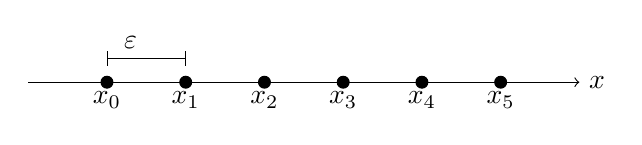
\begin{tikzpicture}
            \draw[->] (-1, 0) -- (6, 0);
            \node[right] at (6, 0) {\(x\)};
            \foreach \x in {0, 1, 2, 3, 4, 5} {
                \draw[fill=black] (\x, 0) circle[radius=0.075cm];
                \node[below] at (\x, 0) {\(x_{\x}\)};
            }
            \draw[|-|] (0, 0.3) -- (1, 0.3);
            \node[above] at (0.3, 0.3) {\(\varepsilon\)};
        \end{tikzpicture}
        \caption{A one dimensional discrete system of \(N = 6\) points, \(x_i\), spaced evenly \(\varepsilon\) apart.}
        \label{fig:one dimensional discrete system}
    \end{figure}
    We can now limit the domain of the wave~function to \(\{x_i\st i=0,\dotsc, 5\}\).
    We define
    \[\psi_i = \sqrt{\varepsilon}\psi(x_i) \in\complex.\]
    We then collect this set of evaluations of \(\psi(x)\) into one object:
    \[
        \ket{\psi} =
        \begin{pmatrix}
            \psi_0\\ \vdots\\ \psi_5
        \end{pmatrix}
    \]
    \(\ket{\psi}\) is a member of a six-dimensional vector space, \(\hilbert\).
    Note that it is wrong to write \(\ket{\psi(x)}\).
    \(\ket{\psi}\) and \(\psi(x)\) are different objects writing \(\ket{\psi(x)}\) is similar to putting a coordinate label on a vector like \(\vv{v}_x\), its just wrong.
    
    \subsubsection{Basis}
    By specifying a vector by its components we assume a basis.
    One such basis is
    \[
        \ket{\xi_0} =
        \begin{pmatrix}
            1\\ 0\\ 0\\ \vdots\\ 0
        \end{pmatrix}
        ,\qquad\ket{\xi_1} =
        \begin{pmatrix}
            0\\ 1\\ 0\\ \vdots\\ 0
        \end{pmatrix}
        ,\dotsc, \ket{\xi_5} =
        \begin{pmatrix}
            0\\ \vdots\\ 0\\ 0\\ 1
        \end{pmatrix}
        .
    \]
    Any vector \(\psi\in\hilbert\) can be written as a linear combination of these basis vectors:
    \[\ket{\psi} = \sum_{k=0}^{5} \psi_k\ket{\xi_k}\]
    where as usual
    \[\psi_k = \braket{\xi_k}{\psi}.\]
    For now we will make some assumptions about extracting physical information from state vectors and wave functions.
    We assume that \(\abs{\psi(x)}^2\) gives the probability density of finding the system at \(x\).
    We also assume that \(\abs{\psi_i}^2 = \varepsilon\abs{\psi(x_i)}^2\) gives the probability of finding the system at \(x_i\).
    Note that the first of these is a probability density and the second is a probability.
    This is because the first is referring to a continuous variable, \(x\), and the second refers to a discrete variable, \(x_i\).
    This is the same as how a probability density function, \(p\), gives a probability, \(p(x)\dd{x}\), here \(\varepsilon\) plays the role of \(\dd{x}\).
    
    With these assumptions we have a physical description of the basis states.
    The vector \(\ket{\xi_i}\) represents a system that is at \(x_i\) with probability 1.
    
    \subsubsection{Scalar Product and Norm}
    We can define a scalar product between \(\ket{\varphi}, \ket{\psi}\in\hilbert\)
    \[\braket{\varphi}{\psi} = \sum_{k=0}^{6} \varphi_k^*\psi_k.\]
    This allows us to induce a norm:
    \[\norm{\psi}^2 = \sum_{k=0}^{6} \abs{\psi_k}^2.\]
    As usual we require state vectors be normalised so
    \[\norm{\psi}^2 = \sum_{k=0}^{6} \abs{\psi_k}^2 = 1.\]
    
    \subsection{Continuous System}
    Moving from this discretised system to a continuous one is as simple as taking the limiting case as \(N \to \infty\) and \(\varepsilon \to 0\).
    After doing this we have that \(\ket{\psi}\in\hilbert_\infty\) where \(\hilbert_\infty\) is an infinite dimensional vector space.
    
    \subsubsection{Basis}
    Define the following basis vectors for our discretised system:
    \[\ket{x_k} = \frac{1}{\sqrt{\varepsilon}}\ket{\xi_k}.\]
    Which gives us \(\ket{\xi_k} = \sqrt{\varepsilon}\ket{x_k}\)
    A vector in the finite dimensional vector space, \(\hilbert\), can be written as
    \[\ket{\psi} = \sum_{k=0}^{N} \psi_k\ket{\xi_k} = \sum_{k=0}^{N} \sqrt{\varepsilon}\psi(x_k)\ket{\xi_k} = \sum_{k=0}^{N} \varepsilon\psi(x_k)\ket{x_k}.\]
    After a limiting process taking \(N\to\infty\) and \(\varepsilon\to 0\) we can write \(\ket{\psi}\in\hilbert_{\infty}\) as
    \[\ket{\psi} = \int\dd{x}\psi(x)\ket{x}\]
    where
    \[\ket{x} = \lim_{\varepsilon\to 0}\frac{1}{\sqrt{\varepsilon}}\ket{\xi_k}.\]
    
    As normal we can find the component, here \(\psi(x)\), with a scalar product with a basis vector:
    \[\psi(x) = \braket{x}{\psi}.\]
    Using this we have
    \[\ket{\psi} = \int\dd{x}\braket{x}{\psi}\ket{x} = \int\dd{x}\ket{x}\braket{x}{\psi}.\]
    We see that \(\ketbra{x}{x}\) is a projection operator and again the completeness relation holds, this time in the form
    \[\int\dd{x}\ketbra{x}{x} = \ident.\]
    
    \subsubsection{Scalar Product and Norm}
    Let \(\ket{\psi}, \ket{\varphi}\in\hilbert\).
    Then their scalar product is
    \[\braket{\varphi}{\psi} = \sum_{k=0}^{N} \varphi_k^*\psi_k = \sum_{k=0}^{N}[\sqrt{\varepsilon}\varphi^*(x_k)][\sqrt{\varepsilon}\psi(x_k)] = \sum_{k=0}^{N}\varepsilon\varphi^*(x_k)\psi(x_k).\]
    After a limiting process taking \(N\to\infty\) and \(\varepsilon\to 0\) we see that for \(\ket{\varphi}, \ket{\psi}\in\hilbert_\infty\) we have
    \[\braket{\varphi}{\psi} = \int\dd{x}\varphi^*(x)\psi(x).\]
    The norm induced by this for \(\ket{\psi}\in\hilbert_\infty\) is given by
    \[\norm{\psi}^2 = \braket{\psi}{\psi} = \int\dd{x}\psi^*(x)\psi(x) = \int\dd{x}\abs{\psi(x)}^2.\]
    For states to be normalisable we require that \(\norm{\psi} < \infty\).
    The space of functions, \(f\colon A\to \complex\), that have this property is called the space of \define{square integrable functions} and is denoted \(\squareIntegrable(A)\).
    For our example of a continuous system we are interested in \(\squareIntegrable(\reals)\).
    If we limit our system to the interval \([a, b]\) where \(a, b\in\reals\) and \(b > a\) then we are interested in the space \(\squareIntegrable([a, b])\).
    
    \subsubsection{Scalar Product of Basis Vectors}
    In the discrete system \(\ket{\xi_k}\) describes a state that is a \(x_k\) with probability 1.
    We want to know what \(\ket{x}\) describes in our continuous case.
    Consider the inner product of two basis states:
    \[\braket{x}{x'} = \lim_{\varepsilon\to 0}\braket{x_k}{x_{k'}} = \lim_{\varepsilon\to 0} \frac{1}{\varepsilon}\braket{\xi_k}{\xi_{k'}}.\]
    Using the orthonormality of \(\{\xi_k\}\) this gives us
    \[
        \braket{x}{x'} = \lim_{\varepsilon\to 0}\frac{1}{\varepsilon}\delta_{kk'} =
        \begin{cases}
            0, & x \ne x',\\
            \infty, &x = x',
        \end{cases}
    \]
    where we have used the fact that if \(x = x'\) then \(\ket{\xi_k} = \ket{\xi_{k'}}\) so \(\delta_{kk'} = \delta_{kk} = 1\) so
    \[\lim_{\varepsilon\to 0} \frac{1}{\varepsilon} = \infty.\]
    On the other hand if \(x \ne x'\) then \(\ket{\xi_k}\ne\ket{\xi_{k'}}\) so \(\delta_{kk'} = 0\).
    Then in the limit we have
    \[\lim_{\varepsilon\to 0}\frac{0}{\varepsilon} = \lim_{\varepsilon\to 0}\frac{\dv{\varepsilon}0}{\dv{\varepsilon}\varepsilon} = \lim_{\varepsilon\to 0}\frac{0}{1} = 0.\]
    We now compute the following integral for reasons that will become clear afterwards:
    \begin{align*}
        \int\dd{x'} f(x')\braket{x}{x'} &= \lim_{\stackrel{N\to \infty}{\varepsilon\to 0}}\sum_{k=0}^{N} \varepsilon f(x_{k'})\braket{x_k}{x_k}\\
        &= \lim_{\stackrel{N\to \infty}{\varepsilon\to 0}}\sum_{k=0}^{N} \varepsilon f(x_{k'})\frac{1}{\varepsilon}\braket{\xi_{k}}{\xi_{k'}}\\
        &= \lim_{N\to\infty}\sum_{k=0}^{N}  f(x_k)\braket{\xi_{k}}{\xi_{k'}}\\
        &= \lim_{N\to\infty} f(x_{k'})\delta_{kk'}\\
        &= \lim_{\varepsilon\to 0}f(x_{k})\\
        &= f(x)
    \end{align*}
    So we see that
    \[\int\dd{x'}f(x')\braket{x}{x'} = f(x)\]
    this, as well as being zero if \(x \ne x'\) defines the \define{Dirac delta distribution}:
    \[
        \delta(x - x') =
        \begin{cases}
            0, & x\ne x',\\
            \infty, & x = x'
        \end{cases}
    \]
    and
    \[\int\dd{x'}f(x')\delta(x - x') = f(x).\]
    So we can identify
    \[\braket{x}{x'} = \delta(x - x').\]
    Using this we get around the fact that \(\{\ket{x}\}\) are not normalisable, that is that \(\braket{x}{x} = \infty\), and we can still extract meaningful information as long as we only have \(\braket{x}{x}\) inside of integrals.
    
    